\documentclass[12pt]{article}
\usepackage[]{cite}
\usepackage{cmap}
\usepackage[T2A]{fontenc}
\usepackage[utf8]{inputenc}
\usepackage[english, russian]{babel}
\usepackage{amsmath, amsfonts,amssymb}
\usepackage{graphicx, epsfig}
% \usepackage{subfig}
\usepackage{subcaption}
\usepackage{color}
\usepackage{hyperref}


% \newcommand\argmin{\mathop{\arg\min}}
% \newcommand{\T}{^{\text{\tiny\sffamily\upshape\mdseries T}}}
% \newcommand{\hchi}{\hat{\boldsymbol{\chi}}}
% \newcommand{\hphi}{\hat{\boldsymbol{\varphi}}}
% \newcommand{\bchi}{\boldsymbol{\chi}}
% \newcommand{\A}{\mathbf{A}}
% \newcommand{\bb}{\mathbf{b}}
% \newcommand{\B}{\mathcal{B}}
% \newcommand{\W}{\mathbf{W}}
\newcommand{\E}{\mathbb{E}}
\newcommand{\x}{\mathbf{x}}
\newcommand{\y}{\mathbf{y}}
\newcommand{\Y}{\mathbf{Y}}
\newcommand{\X}{\mathbf{X}}
\newcommand{\D}{\mathcal{D}}
\newcommand{\s}{\mathbf{s}}
% \newcommand{\Z}{\mathbf{Z}}
% \newcommand{\hx}{\hat{x}}
% \newcommand{\hX}{\hat{\X}}
% \newcommand{\hy}{\hat{y}}
\newcommand{\M}{\mathcal{M}}
\newcommand{\I}{\mathcal{I}}
\newcommand{\Q}{\mathcal{Q}}
\renewcommand{\S}{\mathcal{S}}
% \newcommand{\N}{\mathcal{N}}
\newcommand{\R}{\mathbb{R}}
% \newcommand{\p}{p(\cdot)}
% \newcommand{\cc}{\mathbf{c}}
% \newcommand{\m}{\mathbf{m}}
% \newcommand{\bt}{\mathbf{t}}
% \newcommand{\e}{\mathbf{e}}
% \newcommand{\h}{\mathbf{h}}
% \newcommand{\q}{q(\cdot)}
% \newcommand{\uu}{\mathbf{u}}
% \newcommand{\vv}{\mathbf{v}}
% \newcommand{\dd}{\partial}

\renewcommand{\baselinestretch}{1}


\newtheorem{Th}{Теорема}
\newtheorem{Def}{Определение}
\newenvironment{Proof} % имя окружения
    {\par\noindent{\bf Доказательство.}} % команды для \begin
    {\hfill$\scriptstyle\blacksquare$} % команды для \end
\newtheorem{Assumption}{Предположение}
\newtheorem{Corollary}{Следствие}

\textheight=24cm % высота текста
\textwidth=16cm % ширина текста
\oddsidemargin=0pt % отступ от левого края
\topmargin=-1.5cm % отступ от верхнего края
\parindent=24pt % абзацный отступ
\parskip=0pt % интервал между абзацами
\tolerance=2000 % терпимость к "жидким" строкам
\flushbottom % выравнивание высоты страниц

%\graphicspath{ {fig/} }



\begin{document}

\thispagestyle{empty}
\begin{center}
    \sc
        Министерство образования и науки Российской Федерации\\
        Московский физико-технический институт
        {\rm(государственный университет)}\\
        Физтех-школа прикладной математики и информатики\\
        Кафедра <<Интеллектуальные системы>>\\
        Направление <<Интеллектуальный анализ данных>> \\[30mm]
    \rm\large
        Соболевский Федор Александрович\\
        Б05-111\\[10mm]
    \bf\Large
	Применение больших языковых моделей 
        для иерархической суммаризации
        текстов научных публикаций \\[10mm]
    \rm\normalsize
    \sc
        Выпускная квалификационная работа бакалавра\\[10mm]
\end{center}
\hfill\parbox{90mm}{
    \begin{flushleft}
    \bf
        Научный руководитель:\\
    \rm
        д.~ф.-м.~н. Воронцов Константин Вячеславович\\[5cm]
    \end{flushleft}
}
\begin{center}
    Москва\\
    2025
\end{center}


\newpage
\tableofcontents
\newpage

\begin{abstract}
В век экспоненциального роста количества доступной информации в мире особенно актуальной становится задача структурирования и систематизации научных знаний, а также повышения их доступности. Иерархическая организация основных идей и результатов в научных публикациях может позволить ускорить процесс получения читателем знаний и позволить ему двигаться при изучении темы от главного к деталям. Одним из видов структурированного представления текста являются интеллект-карты из предложений, или иерархические сводки. Поскольку человеческая обработка больших коллекций текстовых документов, особенно научных, занимает много времени и ресурсов, для решения задачи их иерархической суммаризации необходимо разрабатывать автоматические методы, по качеству не уступающие ручной суммаризации. 

Перспективным инструментом решения данной задачи являются большие языковые модели (БЯМ). В данной работе исследуется способность больших языковых моделей строить иерархические представления текстов научных публикаций. Основным методом оценки качества иерархической суммаризации, как и обычной суммаризации, является оценка сходства с эталонной сводкой. Поскольку на данный момент не существует выборок для данной задачи, предварительно создается выборка интеллект-карт по ряду научных статей для сравнения со сгенерированными автоматически. Иерархическая суммаризация с помощью БЯМ оценивается в сравнении с сводками из этой выборки с учетом различных аспектов сходства иерархических сводок, таких как структура, семантика, ранжирование фактов в иерархии и другие.

Применяемые до сих пор методы сравнения текстовых иерархий основаны на сравнении их на лексическом уровне и, как показано в данной работе, слабо учитывают их структуру и семантику. С связи с этим в данной работе предлагается также новый метод сравнения текстовых деревьев~--- расстояние редактирования текстовых деревьев (TTED), основанный на расстоянии редактирования и оценке семантической близости с помощью языковых моделей. Для оценки информативности функции расстояния между текстовыми деревьями как агрегации разных аспектов их различия вводятся $R_S$- и $R_M$-коэффициенты, отражающие относительную чувствительность фукнции сходства к семантическим и структурным различиям текстовых деревьев по отношению к перефразированию предложений в вершинах, а также предлагаются несмещенные оценки на эти коэффициенты по выборкам текстовых деревьев. С помощью этих оценок даётся количественная оценка качества предложенной метрики и ее модификаций в сравнении с использованной до этого.

  \bigskip
  \textbf{Ключевые слова}: \emph{большие языковые модели, иерархическая суммаризация, интеллект-карты, текстовые деревья, расстояние редактирования}
\end{abstract}

\newpage

%%%%%%%%%%%%%%%%%%%%%%%%%%%%%%%%%%%%%%%%%%%%%%%%%%%%%%%%%%%%%%%%%%%%%%%%%%%%%
\section*{Введение}
\addcontentsline{toc}{section}{\protect\numberline{}Введение}

\paragraph{Актуальность темы.} С развитием средств хранения, обработки и передачи информации и накоплением данных человечеством количество информации в мире экспоненциально растет, и научные знания не являются исключением. С увеличением скорости появления новых научных публикаций и одновременным накоплением старых все острее необходимость как в эффективном поиске публикаций, актуальных интересующей теме, так и в эффективном извлечении знаний из них. Поскольку современному исследователю в среднем требуется обработать довольно большой объем научных статей, чтобы получить нужную ему информацию по интересующей теме, возникает потребность в организации информации из публикаций, позволяющей читателю ознакомиться с их содержанием с нужной ему степенью детализации, двигаясь при изучении темы от главного к деталям. 

Методом удовлетворения данной потребности представляется \textit{иерархическая суммаризация} научных публикаций, то есть представление их в виде иерархического структуры, в которой на верхних уровнях иерархии находятся ключевые аспекты исследования, а каждая дочерняя вершина детализирует родительскую. Такое представление знаний информации из научного труда потенциально может позволить изучить его с нужным уровнем детализации по каждому отдельному аспекту исследования и извлечь ровно тот объем информации из него, который необходим читателю. Такое представление знаний также может стать способом повысить доступность научных знаний по теме, с помощью которого можно кратко и доступно разобраться в теме и затем при необходимости изучить интересующие детали.

Представление знаний в виде иерархических карт не является новой идеей. В литературе давно известен термин <<интеллект-карта>> (mind map), обозначающий древовидную карту, иерархически раскрывающую тему от главных понятий к деталям (TO-DO: ссылка на источник). Интеллект-карты показали себя как инструмент, позволяющий улучшить восприятие и запоминание информации \cite{guerrero2015mind}, однако самостоятельное построение интеллект-карты по тексту научной публикации является весьма времязатратным занятием. Автоматическая генерация интеллект-карт по научным статьям представляется способом устранить эту проблему и предоставить удобную для восприятия организацию знаний читателю без дополнительных затрат времени.

В последние годы одним из самых универсальных инструментов для генерации и обработки текста стали большие языковые модели (БЯМ). Выдающиеся способности таких моделей к генерации человекочитаемого текста уже нашли свое применение во многих задачах обработки текстов, в том числе в задаче суммаризации, причем современные БЯМ уже способны показывать в данной задаче результаты, по качеству сопоставимые с человеческими \cite{pu2023summarization}. Несмотря на это, хотя в последние годы появилось небольшое число работ, исследующих способность БЯМ генерировать структурированные представления информации \cite{jain2024structsum}, исследование БЯМ в приложении к задаче иерархической суммаризации еще только предстоит провести. 

Немаловажной частью данного исследования является разработка нового подхода к оцениванию иерархической суммаризации и создание новой выборки для этой цели. Несмотря на наличие ряда работ по теме \cite{christensen2014hierarchical, jain2024structsum, zhang2024coreference, wei2019revealing, hu2021efficient}, иерархическая суммаризация является относительно малоизученной задачей, и на данный момент не существует общепринятых методов оценивания автоматической генерации иерархических сводок, а выборки для этой задачи ограничиваются областью новостных текстов и экстрактивным подходом к иерархической суммаризации. Используемый в последних работах по теме метод сравнения иерархических сводок с экспертными основан, как показано в данном исследовании, слабо отражает значимые различия между иерархическими сводками по сравнению с различиями в формулировках. Это обосновывает необходимость разработки новой метрики сходства текстовых иерархий и нового подхода к оцениванию подобных метрик сходства. 

\paragraph{Цели работы.}

\begin{itemize}
    \item Формализовать задачу автоматической иерархической суммаризации как задачу многокритериальной оптимизации.
    \item Предложить новую агрегированную метрику качества для задачи иерархической суммаризации, отражающую прежде всего значимые различия текстовых иерархий.
    \item Формализовать требования к адекватности метрики на множестве текстовых иерархий как метрики на множестве объектов, обладающих различными аспектами сходства.
    \item Разработать и применить методику построения интеллект-карт по научным текстам с целью формирования выборки для обучения и валидации моделей автоматической иерархической суммаризации.
    \item Применить БЯМ для генерации интеллект-карт по текстам научных статей и определить оптимальный метод работы с моделью, позволяющий максимизировать качество генерации для выбранной БЯМ.
    \item Проанализировать свойства генерируемых с помощью БЯМ карт, их достоинства и недостатки самих по себе и в сравнении со стандартами и определить границы применимости современных БЯМ для иерархической суммаризации научной литературы. 
\end{itemize}

\paragraph{Научная новизна.} 
\textit{TO-DO}

\textit{to my best knowledge, на данный момент нет ни адекватных критериев для автоматического оценивания карт знаний по научным статьям, ни выборки для данной задачи}


\paragraph{Теоретическая значимость.}
\textit{TO-DO}

\textit{- формализация задачи гибридной иерархической суммаризации в виде интеллект-карт из предложений}

\textit{- разработка автоматических метрик оценки качества иерархических представлений текста по собственной структуре карты и в сравнении с референсом}


\paragraph{Практическая значимость.}
\textit{TO-DO}

\textit{- разработка метода автоматической генерации представлений научных статей для их эффективного изучения с нужной степенью углубления в детали}

\textit{- датасет для задачи генерации интеллект-карт из предложений по научным текстам}

\textit{- (было бы неплохо?) фреймворк для автоматического оценивания подобных интеллект-карт}


\paragraph{Степень достоверности и апробация работы.} Результаты работы по разработке метрики TTED на множестве текстовых деревьев были представлены мной на 67-й Всероссийской научной конференции МФТИ в докладе <<Метод оценки сходства текстовых деревьев с помощью расстояния редактирования и языковых моделей>> в секции проблем интеллектуального анализа данных, распознавания и прогнозирования. Весь код, использованный в данной работе для проведения вычислительных экспериментов, находится в открытом доступе для репликации полученных мною результатов по ссылке: \texttt{https://github.com/intsystems/Sobolevsky-BS-Thesis}.

%%%%%%%%%%%%%%%%%%%%%%%%%%%%%%%%%%%%%%%%%%%%%%%%%%%%%%%%%%%%%%%%%%%%%%%%%%%%%
\newpage
\section*{Обозначения и сокращения}
\addcontentsline{toc}{section}{\protect\numberline{}Обозначения}
\begin{itemize}
    \item \textit{БЯМ}~--- большая языковая модель (large language model);
    
    \item Под \textit{иерархическими сводками}, \textit{картами знаний} или \textit{интеллект-картами} в данной работе будут подразумеваться интеллект-карты на основе предложений (salient-sentence-based mind maps, SSM \cite{wei2019revealing}).

    \item \textit{KSM}~--- интеллект-карта на основе главных выдержек (key-snippet based mind map \cite{wei2019revealing}).

    \item \textit{ROUGE} - Recall-Oriented Understudy for Gisting Evaluation (статистическая метрика качества суммаризации).

    \item \textit{BLEU} - Bilingual Evaluation Understudy (статистическая метрика качества генерации текста, основное применение~--- оценка машинного перевода).

    \item \textit{ИАТ}~--- интеллектуальный анализ текста (text mining).

    \item \textit{TED}~--- расстояние редактирования дерева (tree edit distance \cite{zhang1989simple}).
\end{itemize}

%%%%%%%%%%%%%%%%%%%%%%%%%%%%%%%%%%%%%%%%%%%%%%%%%%%%%%%%%%%%%%%%%%%%%%%%%%%%%
\newpage
\section{Постановка задачи}
\subsection{Текстовые иерархии как объект исследования}
Объектом данного исследования являются иерархические сводки текстовых документов. Иерархическая сводка по своей структуре есть ничто иное, как текстовая иерархия, то есть дерево, метками вершин которого являются фрагменты текста. Определим этот объект формально. Пусть задан словарь $\mathcal{W}$ и соответствующее множество $\mathcal{S}$ фрагментов текста, составленных из слов этого словаря: 
$$
\forall s\in\mathcal{S}\quad s = \left(w_j\right)_{j=1}^{|s|}, \quad w_j\in \mathcal{W}.
$$
Определим текстовое дерево как дерево $T = (V, E)$, $E\subset V^2$, где ля каждой вершины $v\in V$ задана текстовая метка $s(v)\in \mathcal{S}$. Обозначим множество рассматриваемых текстовых деревьев как $\mathcal{T}$. Текстовые деревья $T\in \mathcal{T}$ будут объектом генерации и сравнения в данном исследовании. 

\subsection{Задача иерархической суммаризации}
Пусть дан документ (или коллекция документов) $\D$~--- упорядоченный набор предложений из $\S$: $\D = \left(s_i\right)_{i=1}^{|\D|}$, $s_i\in \S$, а также иерархическая сводка $T^*\in\mathcal{T}$ данного документа, построенная экспертом. Пусть также задана метрика качества $\I$ генерации текстовых деревьев $T\in\mathcal{T}$ по документам, в общем случае зависящая от справочной карты $\mathcal{T}^*$ и самого документа $\D$, то есть $\I: (T, T^*, \D) \mapsto x\in\R$. Тогда требуется найти отображение $f: \D \mapsto T \in\mathcal{T}$, максимизирующее данную метрику качества $\I$:
\begin{equation} \label{summarization_objective}
    \I(f(\D), T^*, \D) \longrightarrow \max_{f}.
\end{equation}
В более общем случае можно определить набор метрик $\I_k$ такого вида, отражающих различные аспекты качества генерации иерархической сводки $T$. Из основных аспектов качества иерархической суммаризации можно выделить следующие:
\begin{itemize}
    \item Сходство с экспертной сводкой $T^*$ по таким аспектам, как структура карты, ее смысловое содержание, ранжирование фактов в сводке и др.
    \item Качество сводки $T$ как краткого представления документа $\D$, например, полнота сводки или фактическое соответствие $T$ и $\D$.
    \item Качество сводки самой по себе, например, ее неизбыточность, связность внутри вершин и между вершинами, непротиворечивость, соответствие цели генерации и т.\,д.
\end{itemize}
Пусть задана функция $\mathcal{A}(\I_1, \dots, \I_K): \R^K\longrightarrow \R$, каким-то образом агрегирующая метрики аспектов качества $\I_k$. Тогда оптимизационная задача \eqref{summarization_objective} перепишется в более общем виде как
\begin{equation}
    \mathcal{A}\left(\I_1(f(\D), T^*, \D), \dots, \I_K(f(\D), T^*, \D)\right) \longrightarrow \max_{f}.
\end{equation}

\subsection{Задача оптимизации промптинга БЯМ \textit{(TO-DO: обновить)}}
Основной инструмент оптимизации работы готовой БЯМ без её дополнительного дообучения~--- подбор оптимального текстового запроса для решения задачи (\textit{промптинг}). Поскольку на данный момент нет достаточно быстрых алгоритмов поиска по всему множеству возможных запросов, а полный перебор запросов для каждой модели занимает слишком большое время, отдельной задачей в нашей работе является оптимизация промптинга БЯМ для цели генерации интеллект-карт и в целом.

Пусть дана выборка документов $\X$, языковая модель $f$, карта-стандарт $\M^*$ для заданной цели создания карты и некоторая метрика качества $\I$. Пусть также задано множество возможных запросов $\Q$, таких что вывод модели для каждого $(\D, Q)\in\X\times\Q$ соответствует требуемому формату, и содержащих формулировку цели \textit{(TO-DO: сделать ее отдельным параметром)}, \textit{общую для модели и экспертов} - создателей $\M^*$. Требуется найти оптимальный запрос $Q^*\in\Q$, такой что вывод модели при входе $(\D, Q^*)$ максимизирует метрику $\I$ по выборке $\X$:
$$
Q^* = \arg\max\limits_{Q\in\Q} \frac{1}{|\X|}\sum\limits_{\D\in\X} \I(f(\D, Q), \D, ).
$$
Для эффективного поиска оптимального запроса (\textit{промптинга}) требуется также задать полное и неизбыточное множество запросов $\Q$ и эффективную \textit{стратегию поиска оптимального запроса} в $\Q$.

\subsection{Требования к мере близости текстовых деревьев.} \label{metric_requirements}
Чтобы определить адекватную метрику на множестве текстовых деревьев, мы сформулируем некоторые требования к произвольной метрике в пространстве таких объектов. Пусть задана функция семантической (смысловой) близости текстовых фрагментов: $r: \mathcal{S}^2 \rightarrow [0, +\infty)$. Для вершин $v, v'\in V$ дерева $T=(V, E)$ обозначим $r(v, v') := r(s(v), s(v'))$, а $r(v) := r(s(v), \lambda)$, где $\lambda$~--- пустая строка. Требуется определить функцию сходства $\rho: \mathcal{T}^2 \rightarrow [0, +\infty)$, отвечающую следующим требованиям учета семантической и структурной близости:
\begin{enumerate}
    \item Симметричность: $\rho(T, T') = \rho(T', T)$.
    \item Равенство нулю в случае равенства аргументов: $\rho(T, T) = 0$.
    \item Существует некоторая неубывающая функция $f: [0,+\infty) \rightarrow [0,+\infty)$, такая что:
    \begin{enumerate}
        \item Если $T'$ получено из $T$ добавлением в $T$ вершины $v$, то $\rho(T, T') = f(r(v))$;
        \item Если $T'$ получено из $T$ удалением из $T$ вершины $v$, то $\rho(T, T') = f(r(v))$;
        \item Если $T'$ получено из $T$ заменой вершины $v$ на $v'$, то $\rho(T, T')= f(r(v, v'))$.
    \end{enumerate}
    \item $\rho$ удовлетворяет неравенству треугольника: 
    \begin{equation} \label{metric_requirement_6}
        \forall T, T', T''\in\mathcal{T}\quad \rho(T,T'')\leq\rho(T,T')+\rho(T',T'').
    \end{equation}
\end{enumerate}

Обозначим теперь некоторые требование к существенности различий между текстовыми деревьями, отражаемых функцией их сходства. Во-первых, естественно требовать от метрики, чтобы она отражала различия текстовых деревьев как по своей \textit{семантике} (то есть смысловому содержанию), так и по \textit{структуре}. Во-вторых, информативная метрика должна слабо реагировать на несущественные отличия~--- например, на \textit{парафразирование} предложений в вершинах дерева. Следовательно, среднее значение метрики для деревьев, различающихся по первым двум признакам, должно быть меньше относительно среднего значения расстояния между деревьями, полученными друг из друга парафразированием. 

Формализуем эти требования. Обозначим за $P(T)$ множество деревьев, которые можно получить из $T$ парафразированием его меток, $S(T)$~--- множество деревьев, составленных из того набора вершин с теми же метками, что и $T$ (но отличающихся по структуре), $M(T)$~--- набор деревьев с такой же структурой, как у $T$, но с разной семантикой. Для конкретности определим последнее множество так: $M(T) = \mathcal{T}_{\sim T} \setminus P(T)$, где $\mathcal{T}_{\sim T}$~--- множество деревьев с такой же структурой, как у $T$. Тогда качественные требования, сформулированные выше, будут отражены формально в следующих соотношениях:
\begin{equation} \label{info_requirements}
    \E_{T'\in P(T), \ T''\in S(T)} \left[\frac{\rho(T, T')}{\rho(T, T'')}\right] \ll 1, \quad \E_{T'\in P(T), \ T''\in S(T)} \left[\frac{\rho(T, T')}{\rho(T, T'')}\right] \ll 1 \quad \forall T\in\mathcal{T}.
\end{equation}
Обозначим
\begin{equation} \label{r_coeffs}
    \E_{T'\in P(T), \ T''\in S(T)} \left[\frac{\rho(T, T')}{\rho(T, T'')}\right] := r_S(\rho, T), \quad \E_{T'\in P(T), \ T''\in S(T)} \left[\frac{\rho(T, T')}{\rho(T, T'')}\right] := r_M(\rho, T).    
\end{equation}
Введем коэффициента информативности метрики $\rho$, не зависящие от выбранного дерева $T\in\mathcal{T}$:
\begin{equation} \label{R_coeffs}
    R_S(\rho) = \E_{T\in \mathcal{T}}[r_S(\rho, T)], \quad R_M(\rho) = \E_{T\in \mathcal{T}}[r_M(\rho, T)] 
\end{equation}
Требования \eqref{info_requirements} перепишутся в более простом виде: $R_S(\rho) \ll 1$, $R_M(\rho) \ll 1$. Тогда соответствующие задачи оптимизации, решаемые мной в данной работе, будут выглядеть следующим образом:
\begin{equation} \label{optimization_problem}
     R_S(\rho) \longrightarrow \min_\rho, \quad  R_M(\rho) \longrightarrow \min_\rho.
\end{equation}

%%%%%%%%%%%%%%%%%%%%%%%%%%%%%%%%%%%%%%%%%%%%%%%%%%%%%%%%%%%%%%%%%%%%%%%%%%%
\newpage
\section{Обзор}
\subsection{Методы суммаризации}

\paragraph{Суммаризация текстов и БЯМ.} Задача суммаризации текста представляет из себя задачу получения краткого представления $\S$ документа (или коллекции документов) $\D$. Выделяют два основных вида суммаризации: \textit{экстрактивную} (extractive), использующую предложения исходного документа ($\S\subset\D$), и \textit{абстрактивную} (abstractive), то есть генерацию новых предложений на основе исходного текста ($\S\not\subset\D$). Также отдельно упоминается так называемая \textit{гибридная суммаризация} (hybrid summarization), подразумевающая извлечение из документа важных предложений с последующим их преобразованием \textit{(TO-DO: ссылка на источники терминов)}. 

Хотя задача суммаризации появилась в научной литературе ещё во второй половине XX века \cite{luhn1958automatic}, основной объем работ по суммаризации текстов был опубликован уже в XXI году, причем до начала бурного развития архитектур глубокого обучения основные методы построения сводок документов и их оценки были в большинстве своем экстрактивными, основанными на статистических приемах обработки текстов \cite{allahyari2017text}. Абстрактивная суммаризация начала активно развиваться с момента появления трансформерных архитектур и других архитектур глубокой машинной обработки текста \cite{el2021automatic}. 

Особенных успехов в области удалось добиться с появлением больших языковых моделей, которые стали основным инструментом ля суммаризации текстов, так как показали значения метрик качества, которых до этого момента не удавалось добиться \cite{jin2024comprehensive}. Более того, способности БЯМ к пониманию, обработке и генерации текста нашли свое применение не только для автоматической генерации сводок, но и для их же оценивания и корректировки \cite{wu2023large}. Сравнение результатов работы БЯМ и человека по классической (линейной) суммаризации текстов на данный момент позволяет утверждать, что для некоторых типов текста машинная суммаризация с помощью БЯМ уже достигла уровня человека \cite{pu2023summarization}. Авторы данной работы, однако, подчеркивают, что проблема оценки качества нейросетевой суммаризации и генерации текста в целом до сих пор остается открытой, поэтому нельзя утверждать о полной достаточности БЯМ для суммаризации. Применимость БЯМ для других видов суммаризации текстов все еще остается мало исследованной.

\paragraph{Иерархическая суммаризация.} Идея структурированной суммаризации текстов как более эффективного способа суммаризации больших документов появилась в научной литературе еще в конце 2000-х гг. \cite{yang2008hierarchical}, однако впервые она была формализована в работе \cite{christensen2014hierarchical}. В первоначальной постановке задача иерархической суммаризации текста представляет из себя задачу генерации \textit{иерархии из сводок} по исходной коллекции документов, в которой дочерние сводки раскрывают содержание элементов (например, предложений) более общих сводок. Метод, представленный в \cite{christensen2014hierarchical}, подразумевает иерархическую кластеризацию предложений текста с последующей суммаризацией каждого кластера. Целевая функция в \cite{christensen2014hierarchical} отражает значимость выделенных предложений, неизбыточность и связность (как внутри элементов иерархии, так и между ними) полученной иерархической сводки. Хотя авторам удалось показать, что данный подход к суммаризации новостных текстов более предпочтителен среди пользователей, чем классические подходы к суммаризации новостных текстов, данная методика не получила дальнейшего развития. Более применимыми стали подходы, основанные на генерации \textit{интеллект-карт} на основе текстов.

\paragraph{Интеллект-карты.} На сегодняшний день существует множество различных видов организации знаний в виде графовых структур: онтологии, карты концепций (concept maps) и другие, но в данной работе нас будут интересовать \textit{интеллект-карты}, или \textit{карты знаний}, поскольку они являются наиболее наглядными и удобными для освоения новой информации от главного к деталям. В работах по автоматической генерации интеллект-карт выделяют два основных вида интеллект-карт: \textit{интеллект-карты на основе значимых предложений} (salient sentence-based mind maps, SSM \cite{wei2019revealing}) и \textit{интеллект-карты на основе главных выдержек} (key snippet-based mind maps, KSM\cite{wei2019revealing}). В данной работе нас будут интересовать именно SSM как форма иерархической организации \textit{фактов} (в роли которых будут выступать связные предложения), однако следует подчеркнуть, что практическая значимость интеллект-карт в образовании и других областях исследовалась больше на примере KSM. Также обратим внимание на то, что интеллект-карты при применении их человеком зачастую не ограничиваются лишь иерархиями из текста и могут содержать как более сложные структурные элементы, так и нетекстовые элементы (например, визуальные).

С момента появления в медиа термина <<mind map>> интеллект-карты были экстенсивно изучены как инструмент представления, обработки и систематизации знаний. Многочисленные исследования применения интеллект-карт в школьном и высшем образовании как для презентации информации ученикам/студентам, так и для систематизации полученных знаний им же показали, что такой способ представления информации может заметно улучшить качество восприятия, запоминания и систематизации знаний студентами, в том числе при изучении научной литературы \cite{guerrero2015mind}. Подробный современный обзор применения интеллект-карт в образовании в XXI веке можно найти, например, в \cite{mitra2023tradition}.

\textit{TO-DO: Найти ещё исследований в "многочисленные исследования"}

\paragraph{Автоматическая генерация интеллект-карт.} В последнее десятилетие появился ряд работ по автоматической суммаризации текстов в виде интеллект-карт разных видов при помощи методов машинного обучения. Стоит отметить, что до этого были работы по генерации карт знаний/онтологий по текстам методами ИАТ, но в этих работах фокус больше направлен на моделирование взаимосвязей между отдельными словами/понятиями в тексте, чем между предложениями/фактами, поэтому для нашего исследования данные работы неактуальны.

В работе \cite{wei2019revealing} был предложен метод интеллект-карт (как KSM, так и SSM) по текстам следующим способом: а) с помощью сравнения эмбеддингов предложений строится граф взаимосвязей между ними; б) по графу взаимосвязей строится интеллект-карта нужного вида. Данная идея нашла свое развитие в работе \cite{hu2021efficient}, в которой авторы предложили более эффективный способ превращения графа отношений между предложениями в интеллект-карту с помощью модуля дистилляции графа (graph refinement module). В работе \cite{zhang2024coreference} эта идея была усовершенствована применением вместо графа отношений между предложениями, строящегося по эмбеддингам предложений, графа соотнесенности (coreference graph, discourse graph), строящегося по принципу, описанному в работе \cite{xu2019discourse}. В результате в \cite{zhang2024coreference} были полученные самые высокие значения используемых метрик качества, поэтому мы можем использовать данную модель в качестве базовой для сравнения результатов, полученных с помощью БЯМ, и результатов, достижимых с помощью специализированных нейросетевых архитектур.

В недавнее время были начаты исследования способности БЯМ к генерации подобных интеллект-карт. В работе \cite{jain2024structsum} с помощью промптинга больших языковых моделей строятся так называемые \emph{StructSum}~--- структурированные сводки текстов для поиска конкретной информации, в частности, таблицы и интеллект-карты (KSM). Авторы применяют \textit{самокритики} модели (critics) для улучшения качества генерации, такие как запросы по оцениванию самой моделью различных аспектов качества сгенерированного ею же StructSum и генерация вопросно-ответных пар по исходному тексту для проверки возможности находить нужную информацию из текста в полученной карте. Хотя тот формат карт и решаемые ими задачи, что исследуется в работе \cite{jain2024structsum}, несколько отличается от рассматриваемого в нашей работе, данное исследование подкрепляет предположение о том, что при достаточно изящной стратегии промптинга БЯМ могут дать качественное решение поставленной нами задачи.

\textit{TO-DO: Коммерческие сервисы}

\subsection{Оценка качества суммаризации}
\paragraph{Статистические критерии.} Общепринятым подходом к оцениванию суммаризации с начала развития методов решения данной задачи является использование статистических критериев качества. Самые часто используемые из них, семейство метрик ROUGE \cite{lin2004rouge}, основаны на количестве совпадающих текстовых единиц, таких как n-граммы, последовательности слов и пары слов, между сгенерированной сводкой и экспертным резюме. Другие подобные метрики качества~--- BLEU \cite{papineni2002bleu}, METEOR \cite{banerjee2005meteor}, MoverScore \cite{zhao2019moverscore} и другие~--- схожи с ROUGE по принципу работы в том смысле, что они оценивают сходство стандартной и сгенерированной сводок на уровне слов, словосочетаний, n-грамм и других небольших лексических единиц. 

Основной проблемой вышеперечисленных критериев является низкая репрезентативность статистического подхода в задаче оценки осмысленности, фактичности, связности и других более тонких аспектов сгенерированных сводок. Например, в работе \cite{fabbri2021summeval} по результатам масштабного сравнительного исследования автоматических критериев качества и экспертных оценок искусственно сгенерированных сводок новостных текстов был сделан вывод о том, что экспертные оценки некоторых аспектов реального качества суммаризации, какие как связность и актуальность сводки, достаточно низко коррелируют со значениями автоматических метрик, что указывает на серьезную проблему с автоматическим оцениванием генерации текста статистическими критериями. Это указывает на необходимость использования более сложных критериев качества, учитывающих смысловую структуру исходного текста и его стандартных и искусственно сгенерированных сводок.

\paragraph{Критерии, основанные на БЯМ.}Другим подходом к оцениванию качества суммаризации, ставшим довольно распространенным в последние пять лет, является оценивание суммаризации с помощью БЯМ. Из метрик, основанных на таком подходе, можно выделить BertScore \cite{zhang2019bertscore}, Shepherd \cite{wang2023shepherd} и Booookscore \cite{chang2023booookscore}. Несколько недавних работ также исследуют способность современных моделей по типу GPT оценивать качество суммаризации и искать ошибки в сгенерированных текстах. На данный момент такие методы также не являются полноценным решением проблемы оценивания качества суммаризации в силу неидеальности самих моделей, но они показывают многообещающие результаты. Более подробный обзор этих и других методов оценивания суммаризации с помощью БЯМ можно найти в \cite{jin2024comprehensive}. 
% TO-DO: Обзор БЯМ-методов

Отсутствие достаточно информативных метрик качества суммаризации остается основной проблемой в области суммаризации на сегодня. Во многих современных работах по автоматической суммаризации до сих пор используются простые статистические метрики по типу ROUGE и BLEU, причем зачастую смысл этих метрик не раскрывается, что делает сложным оценку реального качества генерируемых сводок. Хотя некоторыми исследователями были предприняты попытки систематического переосмысления оценивания качества суммаризации \cite{fabbri2021summeval}, \cite{zhang2024benchmarking}, на сегодняшний день задача разработки достаточных метрик для полного, разностороннего автоматического оценивания качества суммаризации остается нерешенной.

\paragraph{Определение семантического сходства.} На сегодняшний день лучшие результаты при решении задач оценки семантической близости предложений и детектирования парафраз были достигнуты с использованием моделей на основе трансформерных архитектур; в частности, с использованием моделей на основе энкодера BERT и им подобных \cite{chandrasekaran2021evolution, vrbanec2023comparison}. \textit{TO-DO: более подробный обзор}

\paragraph{Сравнение иерархий.} \textit{TO-DO: параграф про метрики, с помощью которых сравнивают деревья.}

\paragraph{Оценивание иерархической суммаризации.} Стандартным подходом к оценке качества генерации иерархических сводок, как и в целом в суммаризации, является сравнение полученной сводки со сводкой, созданной по тому же документу экспертом. В силу того, однако, что число работ по теме иерархической суммаризации на данный момент невелико, общепринятой метрики для сравнения текстовых иерархий не существует, что затрудняет сравнение различных подходов к решению задачи иерархической суммаризации. Иерархическая сводка представляет собой дерево из текста, и потому адекватное сравнение таких объектов должно быть многокритериальным и учитывать как семантику предложений в вершинах, так и структуру иерархии. 

В имеющихся на данный момент работах по данной теме текстовые деревья, как правило, сравниваются отдельно по своей структуре как деревья и отдельно с помощью, например, метрики ROUGE \cite{lin2004rouge} как наборы текста \cite{wei2019revealing, zhang2024coreference}. Такой подход, однако, не учитывает взаимосвязь между структурой текстового дерева и его содержанием, а применение статистических метрик по типу ROUGE все еще может не учитывать семантические сходства/различия текста \cite{fabbri2021summeval}. \textit{TO-DO: описать подробнее существующие методы.} 

\textit{TO-DO:}

\textit{- Секция обзора про промптинг}

%%%%%%%%%%%%%%%%%%%%%%%%%%%%%%%%%%%%%%%%%%%%%%%%%%%%%%%%%%%%%%%%%%%%%%%%%%%%%%
\newpage
\section{Предлагаемый метод}

\subsection{Метрика для сравнения текстовых деревьев}

Проанализируем требования к метрике для сравнения текстовых деревьев, сформулированные в разделе \ref{metric_requirements}. Из последнего условия \eqref{metric_requirement_6} естественным образом следует, что расстояние $\rho$ будет соответствовать наименьшему по стоимости набору операций редактирования дерева, так как в противном случае последнее условие можно будет тривиально нарушить. Также отмечу, что, во-первых, заданная таким образом функция $\rho$ будет являться метрикой, коль скоро метрикой является $f\left(r(\cdot, \cdot)\right)$, и, во-вторых, заданным требованиям тривиально удовлетворяет расстояние редактирования деревьев (tree edit distance, TED) со стоимостями операций редактирования, заданными в соответствием с выдвинутыми требованиями.

Для вычисления TED мы будем применять алгоритм Zhang-Shasha, а именно его модификацию для неупорядоченных деревьев \cite{zhang1992editing}. В качестве стоимости обновления вершины, то есть замены фрагмента текста в вершине на другой, исходя из требований к метрике выше естественно использовать степень семантического сходства этих фрагментов, то есть степень их сходства по смыслу. На данный момент, однако, не существует ни общепринятой меры семантической близости предложений, ни алгоритма для ее автоматического вычисления, поэтому для практического воплощения предлагаемого метода нам придется оценивать степень семантического сходства. Для этого мы предлагаем использовать в качестве оценки расстояние между эмбеддингами заданных предложений, полученными с помощью заранее выбранной языковой модели. 

Пусть имеется языковая модель $\text{LM}: S \rightarrow \R^n$, сопоставляющая фрагментам текста некоторые конечномерные эмбеддинги. Тогда мы можем определить для $s, s'\in\mathcal{S}$ семантическое расстояние как $r(s, s') = \rho_n(\text{LM}(s), \text{LM}(s'))$, где $\rho_n$~--- функция расстояния в $\R^n$. В качестве меры семантической близости эмбеддингов можно использовать, например, косинусный коэффициент (cosine similarity) $S_C$ \cite{vrbanec2023comparison}. В таком случае функцию расстояния естественно определить как $\rho_n(A, B) = 1 - S_C(A, B)$.

\paragraph{Модификации алгоритма}
Для усовершенствования полученного алгоритма мы предлагаем несколько эвристических модификаций.
\begin{enumerate}
    \item \textbf{Использование контекста.} Зачастую на практике некорректно сравнивать предложения в вершинах дерева без учета их контекста. Например, предложения «В статье рассказывается про него.» и «В статье рассказывается про метод сравнения текстовых деревьев.» фактически эквивалентны, если в родительской вершине первого стоит предложение «Предлагается новый метод сравнения текстовых деревьев.». В связи с этим в своей реализации мы добавляем возможность при сравнении деревьев предварительно добавлять в метки вершин все предложения из родительских вершин в качестве контекста перед предложением в вершине и после сравнивать эмбеддинги, полученные с помощью модели с учетом этого контекста.
    \item \textbf{Фактор глубины.} В зависимости от приложения предложенного алгоритма различие предложений в листьях дерева и в вершинах, близких к корневой, может считаться более или менее значимым. В связи с этим мы определяем коэффициент глубины $\gamma$, позволяющий изменять вес степени сходства между предложениями в вершинах в зависимости от их глубины: $f(r(v, v')) = \gamma^d r(v, v')$, где $d$~--- глубина вершины $v$.
    \item \textbf{Предварительное вычисление.} Многократное вычисление эмбеддингов с помощью нейросетевой модели может быть очень затратно по времени для больших деревьев, поэтому мы предлагаем предварительно вычислять эмбеддинги для всех предложений в вершинах и применять предложенный алгоритм уже для дерева из эмбеддингов с вышеуказанной стоимостью обновления меток.
\end{enumerate}

\paragraph{Базовый метод.} Для сравнения с предложенной метрикой я использую функцию сходства текстовых деревьев, использованную в работе \cite{zhang2024coreference} для оценки сходства автоматически сгенерированных интеллект-карт с эталонными. Для текстовых деревьев $T=(V, E)$ и $T'=(V',E')$ функция сходства определяется как:
$$
\text{Sim}(T, T') = \min\limits_{P\subset E\times E'} \sum\limits_{(e, e')\in P}\left(\text{ROUGE}(e_0, e'_0) + \text{ROUGE}(e_1, e_1')\right).
$$
где $P$~--- однозначное сопоставление ребер $T$ ребрам $T'$, ROUGE$(v, v')$~--- усредненная оценка ROUGE-1, ROUGE-2 и ROUGE-L сходства $s(v)$ и $s(v')$:
$$
\text{ROUGE}(e, e') = \frac{1}{3}\left(\text{ROUGE-1}(e_1, e_1')+\text{ROUGE-2}(e_1, e_1')+\text{ROUGE-L}(e_1, e_1')\right).
$$
Поскольку предлагаемый нами метод оценивает расстояние между текстовыми аргументами, а baseline-метод оценивает их сходство, то дл единообразия в качестве функции расстояния для сравнения мы будем использовать $\rho_0(T, T') = \text{Sim}^{\text{max}}-\text{Sim}(T, T')$, где $\text{Sim}^{\text{max}}$~--- максимально возможное значение близости для дерева заданного размера, равное близости идентичных деревьев: $\text{Sim}^{\text{max}} = \text{Sim}(T, T)$.

\subsection{Оценивание качества метрик}

Качество метрики $\rho$ на заданном множестве текстовых деревьев $\mathcal{T}$ в постановке задачи \eqref{optimization_problem} будет определяться по коэффициентам $R_S(\rho)$ и $R_M(\rho)$. Очевидно, что вычислить эти величины в точности не представляется возможным, поскольку перебор всех возможных текстовых деревьев является невыполнимой задачей даже в классе деревьев с заданной максимальной глубиной. Для решения этой проблемы можно воспользоваться оценками, полученными с помощью сэмплирования деревьев $T$ из $\mathcal{T}$ и их модификаций из $P(T)$, $S(T)$ и $M(T)$.

Рассмотрим выборку $\mathcal{D} = \{T, T'_1, \dots, T'_p, T''_1, \dots, T''_s, T'''_1, \dots, T'''_m\}$, где $T\sim \mathcal{T}$, $T'_i\sim P(T)$, $T''_j\sim S(T)$, $T'''_k\sim M(T)$. Введем следующие оценки на $R_S(\rho)$ и $R_M(\rho)$ по $\mathcal{D}$:
$$
R^\mathcal{D}_S(\rho) = \frac{1}{sp}\sum\limits_{i=1}^p\sum\limits_{j=1}^s\frac{\rho(T, T'_i)}{\rho(T, T_j'')},
\quad R^\mathcal{D}_S(\rho) = \frac{1}{mp}\sum\limits_{i=1}^p\sum\limits_{k=1}^m\frac{\rho(T, T'_i)}{\rho(T, T_k''')}.
$$
Положим, что введенные в постановке задачи величины $r_S(\rho, T)$, $r_M(\rho, T)$, $R_S(\rho)$, $R_M(\rho)$ корректны для выбранной метрики $\rho$ и класса текстовых деревьев $\mathcal{T}$. Тогда нетрудно видеть, что оценки $R_S(\rho)$ и $R_M(\rho)$ по выборке $\mathcal{D}$ будут несмещенными:
\begin{Th}[Соболевский, 2025]
    Пусть для заданного класса текстовых деревьев $\mathcal{T}$ и метрики $\rho: \mathcal{T}\times\mathcal{T}\longrightarrow [0, +\infty)$ существуют конечные $R_S(\rho)$ и $R_M(\rho)$. Тогда $R_S^\mathcal{D}(\rho)$ и $R_M^\mathcal{D}(\rho)$ являются несмещенными оценками $R_S(\rho)$ и $R_M(\rho)$ соответственно по выборке $\mathcal{D}$:
    $$
    \E_\mathcal{D}[R_S^\mathcal{D}(\rho)] = R_S(\rho), \quad \E_\mathcal{D}[R_M^\mathcal{D}(\rho)] = R_M(\rho).
    $$
\end{Th}
\begin{Proof}
    Здесь приводится доказательство для $R^\mathcal{D}_S(\rho)$, однако доказательство для второго оценки является точно таким же с точностью до переобозначения. Распишем математическое ожидание по выборке $\mathcal{D}$ через математические ожидания по ее элементам, пользуясь свойством условного математического ожидания:
    $$
        \E_\mathcal{D}[R_S^\mathcal{D}(\rho)] = 
        \E_{T\sim \mathcal{T}}\left[\E_{T_i'\sim P(T), \ T_j''\sim S(T)}\left[\left.\frac{1}{sp}\sum\limits_{i=1}^p\sum\limits_{j=1}^s\frac{\rho(T, T'_i)}{\rho(T, T_j'')} \right| T \right]\right].
    $$
    Далее, из линейности математического ожидания
    $$
        \E_{T_i'\sim P(T), \ T_j''\sim S(T)}\left[\left.\frac{1}{sp}\sum\limits_{i=1}^p\sum\limits_{j=1}^s\frac{\rho(T, T'_i)}{\rho(T, T_j'')} \right| T \right] = \left.\frac{1}{sp}\sum\limits_{i=1}^p\sum\limits_{j=1}^s\E_{T_i'\sim P(T), \ T_j''\sim S(T)}\left[\frac{\rho(T, T'_i)}{\rho(T, T_j'')} \right| T \right].
    $$
    Несложно видеть, что под знаком суммы стоит ничто иное, как выражение для $r_S(\rho, T)$. Следовательно,
    $$
        \E_\mathcal{D}[R_S^\mathcal{D}(\rho)] = \frac{1}{sp}\sum\limits_{i=1}^p\sum\limits_{j=1}^s \E_{T\sim \mathcal{T}}[r_S(\rho, T)] = \E_{T\sim \mathcal{T}}[r_S(\rho, T)]  = R_S(\rho),
    $$
    где последнее равенство есть просто определение $R_S(\rho)$.
\end{Proof}

Имея выборку $\mathcal{D}$ обозначенного выше вида и несмещенные оценки $R_S(\rho)$ и $R_M(\rho)$ по ней, можно переписать оптимизационные задачи \eqref{optimization_problem} в следующем виде:
\begin{equation} \label{optimization_problem_2}
    R_S^\mathcal{D}(\rho) \longrightarrow \min_\rho, \quad R_M^\mathcal{D}(\rho) \longrightarrow \min_\rho.
\end{equation}

\subsection{Многокритериальное сравнение интеллект-карт}
Использование агрегированной метрики сходства удобно тем, что упрощает задачу оптимизации генерации текстовых деревьев, однако оно не является способом получить информацию об отличии и сходстве генерируемых интеллект-карт с авторскими по каждому аспекту сходства отдельно. В связи с этим воспользуемся несколькими метриками сходства интеллект-карт, каждая из которых будет отражать аспекты сходства своей природы. Выделим три основных аспекта, по которым будем сравнивать текстовые деревья отдельно:
\begin{enumerate}
    \item \textit{Семантика} дерева, то есть его смысловое содержание в отрыве от древовидной структуры;
    \item \textit{Структура} дерева без учета текстовых меток вершин;
    \item \textit{Ранжирование} фактов в дереве, то есть распределение предложений в вершинах по уровням иерархии.
\end{enumerate}

\paragraph{Семантическое сходство.} Первый измеряемый в данной работе аспект сходства предполагает сходство текстов в вершинах деревьев по смыслу как наборов предложений без графовой структуры. Здесь целесообразно применить одну из метрик, используемых для оценки качества обычной, линейной суммаризации. Среди метрик сходства текста наиболее информативными по определению семантической близости являются методы, основанные на нейросетевом моделировании предложений. Применим одну из таких метрик~--- \textit{BERTScore} \cite{zhang2019bertscore}, основанную на сравнении предложений по их представлениям, полученным с помощью BERT-подобной языковой модели. 

\paragraph{Структурное сходство.} Второй аспект, по которому можно сравнивать интеллект-карты~--- их структура. Для сравнения структур текстовых деревьев можно абстрагироваться от меток их вершин и сравнивать их как неразмеченные деревья. Существуют разные метрики сравнения иерархий, однако остановимся на метрике, которая уже была применена в данной работе и которая нашла широкое применение для сравнения деревьев~--- \textit{расстоянии редактирования}. В данном случае способом сравнить исключительно структуры деревьев будет применить алгоритм поиска расстояния редактирования для них, заменив все метки на одинаковые и задав лишь стоимости операций удаления и добавления вершины равными фиксированному числу~--- например, 1. Тогда заданное таким образом расстояние редактирования будет показывать, сколько операций редактирования минимально необходимо совершить, чтобы получить из структуры первого дерева структуру второго. 

\paragraph{Сходство ранжирования.} Третий выделяемый в данном разделе аспект сходства иерархий~--- сходство в ранжировании предложений в вершинах по уровням иерархии. В терминах оценки качества иерархической суммаризации это означает качество расположения фактов, выносимых в иерархическую сводку, по порядку от главного к деталям. Сразу применить для оценки ранжирования стандартные метрики качества здесь мешают две особенности задачи. Во-первых, предложения в сгенерированной и авторской сводках почти наверное будут отличаться формулировками, хотя могут при этом совсем не отличаться по смыслу. Во-вторых, следует учесть, что на одном уровне иерархии в дереве могут находиться несколько вершин, поэтому нужно учесть нахождение на одном месте в рейтинге сразу многих вершин.

Первую проблему можно решить, сопоставив попарно по семантической близости предложения в вершинах двух деревьев и найдя в них пары ближайших по смыслу предложений, а затем оценивая ранжирование предложений по экспертному ранжированию их пар. Здесь возникает очевидный вопрос: насколько семантически близкими должны быть предложения, чтобы их можно было сопоставить друг другу как один и тот же факт? Для получения четкого ответа на этот вопрос пришлось бы обучать границу отсечения на выборке для задачи детекции парафразов, однако для целей данной работы можно воспользоваться значениями, уже подобранными в работе \cite{vrbanec2023comparison} для используемых языковых моделей.

Для сравнения ранжирования тех предложений во втором дереве, для которых мы нашли соответствующие предложения в первом, можно воспользоваться \textit{коэффициентом ранговой корреляции Спирмена} \cite{spearman1904proof}. При этом предложения, которым не будет найдено соответствие в другом дереве, не будем учитывать при подсчете, поскольку полноту иерархической сводки уже будет оценивать метрика семантического сходства.

\textit{TO-DO: как минимум, отдельный раздел про то, как мы будем пытаться последовательными промптами заставить БЯМ генерировать карты} 

%%%%%%%%%%%%%%%%%%%%%%%%%%%%%%%%%%%%%%%%%%%%%%%%%%%%%%%%%%%%%%%%%%%%%%%%%%%%%%
\newpage
\section{Вычислительные эксперименты}
\subsection{Тестирование метрики для сравнения текстовых деревьев}
\paragraph{Постановка эксперимента.}  
Для проверки применимости предложенной метрики сходства текстовых деревьев в сравнении с ьазовым методом проведем вычисление оценок расстояния на выборке $\mathcal{D}$, состоящей из следующих элементов:
\begin{enumerate}
    \item текстового дерева $T$;
    \item деревьев, которые идентичны по семантическому значению и структуре, но предложения в узлах дерева \textit{перефразированы}~--- подвыборка $\mathcal{T}_1$ из $P(T)$;
    \item деревьев, которые сформированы из одних и тех же предложений, но с разной \textit{структурой} дерева~--- подвыборка $\mathcal{T}_2$ из $S(T)$;
    \item деревьев, которые идентичны по структуре и схожи по наборам слов в предложениях, но значительно \textit{отличаются по значению}~--- подвыборка $\mathcal{T}_3$ из $M(T)$.
\end{enumerate}
Цель~--- найти среди предложенных такую метрику $\rho$, для которой будут минимальными оценки $R_S^\mathcal{D}(\rho)$ и $R_M^\mathcal{D}(\rho)$ согласно задачам минимизации \eqref{optimization_problem_2}. Введу также обозначение $\overline{\rho}_i$ для среднего расстояния между $T$ и деревьями из подвыборки $\mathcal{T}_i$. Тогда качественным признаком информативности метрики $\rho$ будет значительное отличие в меньшую сторону соответствующего значения $\overline{\rho}_1$ от соответствующих значений $\overline{\rho}_2$ и $\overline{\rho}_3$.

\paragraph{Экспериментальные данные.} Поскольку привлечь других экспертов или краудсорсинг к созданию выборки для данной работы не представилось возможным, а ручное создание интеллект-карт занимает довольно много времени, для создания выборки для тестирование метрик на чувствительность к различным аспектам сходства текстовых деревьев был привлечен генеративный ИИ. Процесс генерации данных состоял из следующих этапов:
\begin{enumerate}
    \item Создание базовой интеллект-карты по научному исследованию вручную.
    \item Генерация парафразов, реструктуризаций и переосмыслений этой интеллект-карты при помощи запросов к БЯМ DeepSeek V3 (TO-DO: ссылка на модель).
    \item Ручная проверка сгенерированных данных на соответствие запросу.
\end{enumerate}
Такая методика генерации данных позволила значительно сократить затрачиваемое на создание выборки время в условиях самостоятельной работы и избежать смещения в данных, обусловленного работой одного эксперта, при этом сохраняя контроль качества искусственно сгенерированных данных.

\paragraph{Результаты.} Результаты тестирования различных языковых моделей с расстоянием на основе косинусного коэффициента в сравнении с baseline-методом представлены в таблице~\ref{tab:model_results}. Оценки расстояния, полученные с помощью baseline-алгоритма и нашего алгоритма с использованием модели \texttt{paraphrase-multilingual-mpnet-base-v2} из библиотеки \texttt{sentence\_transformers} представлены на рис.~\ref{fig:baseline} и \ref{fig:results} соответственно. На примере версии TTED с языковой моделью MPNet были проведены эксперименты с разными эмбеддинговыми расстояниями и без использования контекста при вычислении эмбеддингов. Результаты этих экспериментов представлены в таблице~\ref{tab:modification_results}. 

\begin{figure}[h]
\begin{subfigure}{.45\textwidth}
    \centering
    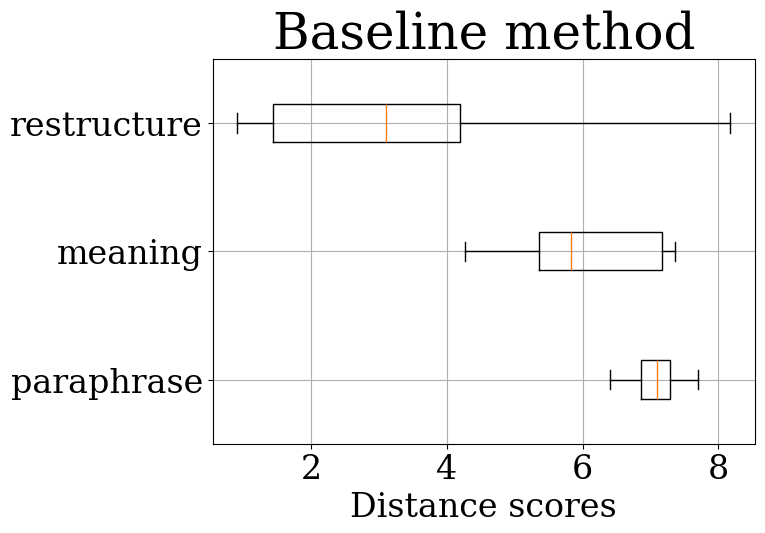
\includegraphics[width=\linewidth]{img/baseline_results.png}
    \caption{Оценки базового метода}
    \label{fig:baseline}
\end{subfigure}~
\begin{subfigure}{.5\textwidth}
    \centering
    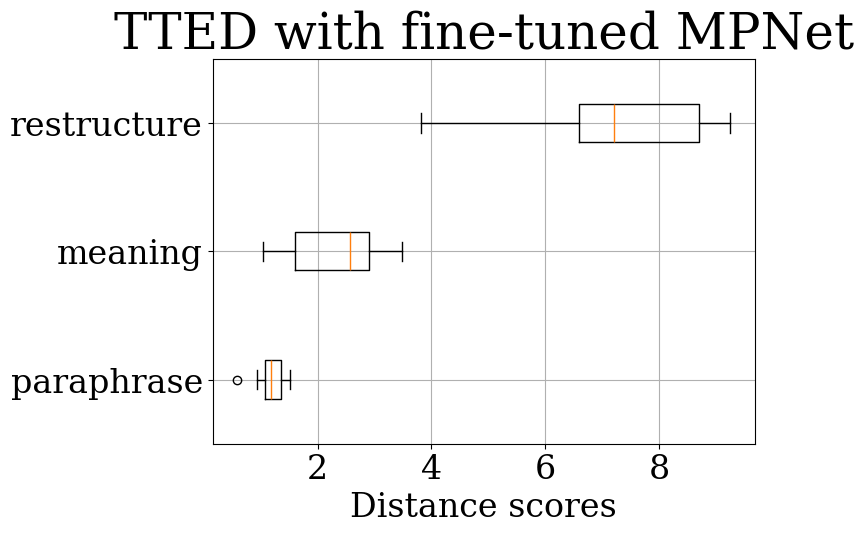
\includegraphics[width=\linewidth]{img/paraphrase_mpnet_results.png}
    \caption{Оценки TTED}
    \label{fig:results}
\end{subfigure}
\caption{Оценки расстояний с помощью TTED и baseline-метода}
\end{figure}

\begin{table}[h]
    \centering
    \begin{tabular}{c|c|c|c|c|c}
        Модель & $\overline{\rho}_1$ & $\overline{\rho}_2$ & $\overline{\rho}_3$ & $R_S^\mathcal{D}(\rho)$ & $R_M^\mathcal{D}(\rho)$ \\ \hline
        Baseline & 7,41$\pm$0,22 & 1,50$\pm$0,71 & 6,25$\pm$0,96 & 6,29$\pm$3,58 & 1,22$\pm$0,24 \\ \hline
        DistilRoBERTa & 2,38$\pm$0,35 & 6,68$\pm$1,66 & 2,83$\pm$0,59 & 0,38$\pm$0,11 & 0,89$\pm$0,28 \\ \hline
        SPECTER & 0,76$\pm$0,21 & 1,96$\pm$0,56 & 0,91$\pm$0,34 & 0,41$\pm$0,14 & 0,92$\pm$0,27 \\ \hline
        MPNet & 1,72$\pm$0,60 & 6,33$\pm$1,76 & 1,87$\pm$0,74 & 0,27$\pm$0,07 & 1,07$\pm$0,59 \\ \hline
        Paraphrase MPNet & 1,35$\pm$0,38 & 6,51$\pm$1,70 & 1,68$\pm$0,56 & \textbf{0,21$\pm$0,05} & \textbf{0,88$\pm$0,37}
    \end{tabular}
    \caption{Средние оценки расстояния с помощью разных языковых моделей}
    \label{tab:model_results}
\end{table}

Видно, что TTED в среднем показывает значения расстояния больше для деревьев, различающихся по семантике и структуре, чем для деревьев, которые являются перефразированием друг друга. По рис.~\ref{fig:results} и значениям $R_2(\rho)$ в таблице~\ref{tab:model_results} видно, что TTED сильнее всего отражает различия деревьев по своей структуре, однако в ходе экспериментов удалось подобрать такую языковую модель \textit{(TO-DO: ссылка на модель)} для построения эмбеддингов, с использованием которой разница между $\overline{\rho}_1$ и $\overline{\rho}_3$ значительна (области значений расстояний на $\mathcal{T}_1$ и $\mathcal{T}_3$ различимы в пределах своих среднеквадратичных отклонений). Это подкрепляет утверждение о том, что TTED отражает значимые отличия текстовых деревьев заметно сильнее, чем незначительные.

Для сравнения рассмотрим значения, полученные с помощью базового метода (рис.~\ref{fig:baseline}, таблица~\ref{tab:model_results}). Мы видим картину, практически противоположную полученной с помощью TTED: наибольшие средние значения расстояний получены между деревьями-парафразами, в то время как расстояния между деревьями с разной структурой, хоть и имея довольно большой разброс, в среднем меньше остальных. Это связано с тем, что в основании базового метода лежит метрика ROUGE, оперирующая на уровне слов и словосочетаний, но не учитывающая реальную семантику предложений, из-за чего более неочевидные смысловые различия не так увеличивают значение расстояния, как перефразирование с изменением большей части слов предложений. Данный эксперимент показывает, что базовый метод сравнения текстовых деревьев отражает значимые отличия деревьев не лучше, чем незначительные.

\begin{table}[h]
    \centering
    \begin{tabular}{c|c|c|c}
        $r(x, y)$ & $\overline{\rho}_1$ & $\overline{\rho}_3$ & $R_M^\mathcal{D}(\rho)$ \\ \hline
        $1 - S_C(x, y)$ & 1,35$\pm$0,38 & 1,68$\pm$0,56 & \textbf{0,88$\pm$0,37} \\ \hline
        $||x-y||_2$ & 13,79$\pm$2,14 & 15,17$\pm$2,45 & 0,93$\pm$0,20 \\ \hline
        $||x-y||_1$ & 291,28$\pm$44,43 & 322,24$\pm$51,94 & 0,92$\pm$0,19
    \end{tabular}
    \caption{Средния значения TTED для разных эмбеддинговых расстояний}
    \label{tab:modification_results}
\end{table}

\textit{TO-DO: поставить новый эксперимент по вычислению времени работы}
% Время работы использованных алгоритмов, включая TTED с предподсчетом и без него, представлено в таблице~\ref{tab:compute_time}.

% \begin{table}[h]
%     \centering
% \begin{tabular}{c|c}
%     Метод & Время вычисления, с \\ \hline
%     TTED без предподсчёта & 554,40  \\ \hline
%     TTED с предподсчётом & \textbf{2,18} \\ \hline
%     Baseline & 3,11
% \end{tabular}
%     \caption{Время работы использованных методов на тестовых данных}
%     \label{tab:compute_time}
% \end{table}
        
%%%%%%%%%%%%%%%%%%%%%%%%%%%%%%%%%%%%%%%%%%%%%%%%%%%%%%%%%%%%%%%%%%%%%%%%%%%%%%
\newpage
\section*{Заключение}
\addcontentsline{toc}{section}{\protect\numberline{}Заключение}

\textit{TO-DO:}
\paragraph{\textit{Обсуждение результатов.}}
\paragraph{\textit{Ограничения исследования.}}
\paragraph{\textit{Направления дальнейшей работы.}}

\paragraph{Основные положения, выносимые на защиту.}
\begin{itemize}
    % ПРЕДЛОЖЕНО: критерий качества метрик на множестве текстовых деревьев
    % ОБЕСПЕЧИВАЮЩЕЕ: возможность оценить информативность метрики  
    % ОТЛИЧАЮЩЕЕСЯ: учет специфики текстовых деревьев как объектов сравнения, обладающих структурой и семантикой
    % +    
    % ПРЕДЛОЖЕНО: оценка на коэффициент качества метрики
    % ОБЕСПЕЧИВАЮЩЕЕ: возможность оценить коэффициент качества метрики по выборке текстовых деревьев
    % ОТЛИЧАЮЩЕЕСЯ: несмещенностью в пространстве текстовых деревьев
    \item Введен новый коэффициент качества метрик на множестве текстовых деревьев, позволяющий оценить информативность метрики как функции расстояния, учитывающей их структуру и семантику, и предложена несмещенная оценка данного коэффициента по выборке текстовых деревьев.
    % ПРЕДЛОЖЕНО: алгоритм сравнения текстовых деревьев
    % ОБЕСПЕЧИВАЮЩЕЕ: агрегированную оценку степени различия между ними 
    % ОТЛИЧАЮЩЕЕСЯ: большей чувствительностью к различиям в семантике и структуре дерева, чем к различиям в формулировке
    \item Разработан новый алгоритм оценки расстояния между текстовыми деревьями, позволяющий агрегировать различные аспекты различия текстовых деревьев и лучше отражающий значимые отличия текстовых деревьев в терминах введенного коэффициента качества, чем используемые до этого методы.
    % ПРЕДЛОЖЕНО: исследование различных методов иерархической суммаризации с помощью БЯМ
    % ОБЕСПЕЧИВАЮЩЕЕ: оценку их применимости в этой задаче
    % ОТЛИЧАЮЩЕЕСЯ: разносторонним анализом результатов генерации в сравнении с валидационными данными
    \item \textit{(в процессе)} Проведено многокритериальное исследование нескольких методов иерархической суммаризации при помощи больших языковых моделей с использованием предложенных новых методов сравнения текстовых деревьев как методов сравнения сгенерированных текстовых иерархий с экспертными.
\end{itemize}

%%%%%%%%%%%%%%%%%%%%%%%%%%%%%%%%%%%%%%%%%%%%%%%%%%%%%%%%%%%%%%%%%%%%%%%%%
\newpage
\addcontentsline{toc}{section}{\protect\numberline{}Список литературы}
\bibliographystyle{ugost2008}
\bibliography{citations}

\end{document}


%%%%%%%%%%%%%%%%%%%%%%%%%%%%%%%%%%%%%%%%%%%%%%%%%%%%%%%%%%%%%%%%%%%%%%%%%%
% ARCHIVE
%%%%%%%%%%%%%%%%%%%%%%%%%%%%%%%%%%%%%%%%%%%%%%%%%%%%%%%%%%%%%%%%%%%%%%%%%%

% \subsection{Методология исследования \textit{(TO-DO: актуализировать)}}

% \paragraph{Сбор экспериментальных данных.} Для проверки работы БЯМ над задачей генерации интеллект-карт по научным публикациям необходима выборка таких карт, созданных людьми с достаточными компетенциями в данной задаче. Для этого и для отработки методики и целей построения иерархических сводок по научным документам первоначальна необходимо проведение самостоятельной работы по построению иерархических сводок научных статей. Предполагается создание набора первоначальных карт, в ходе построения которых, во-первых, должны быть установлены принципы, которыми следует руководствоваться при создании карты знаний, и, во-вторых, должны быть определены цели создания таких карт. Сформулируем несколько примерных целей создания карты знаний по научной публикации~--- получение минимальных знаний, необходимых для:
% \begin{itemize}
% \item воспроизведения результатов авторов статьи студентом или младшим научным сотрудником, разбирающимся в предметной области на базовом уровне;
% \item выделения наиболее важного, нового, значимого результата для его популяризации или включения в образовательный курс по предметной области данного исследования;
% \item выделения основного результата для упоминания в научном обзоре по предметной области;
% \item подготовки пересказа статьи на научном семинаре, максимально близкого к тому, что могли бы рассказать сами авторы, желая донести свои результаты до профессионального сообщества в своей предметной области. 
% \end{itemize}
% Вполне естественно, что данными целями спектр применимости карт знаний не ограничивается, но для определенности в нашем исследовании мы зафиксируем именно их.

% \paragraph{Агрегация экспертных мнений.} Так как мнения экспертов по поводу оптимальных способов построения карт знаний могут разниться, эти мнения нужно агрегировать. Мы предлагаем следующую методику объединения экспертных усилий для совместного создания интеллект-карт по научным текстам: проведение научных семинаров в формате обсуждения интеллект-карт по статьям с последующим построением общей карты. Пусть мы собрали $N$ экспертов и задали $K$ целей создания интеллект-карты, тогда на выходе мы имеем по каждой обработанной статье $N+К$ карт, $K$ из которых выбираются нами в качестве стандартных для дальнейших исследований.

% \paragraph{Отбор критериев качества.} Вышеупомянутые научные семинары можно использовать не только с целью создания стандартных интеллект-карт, но и для сбора экспертных оценок аспектов качества человеческих и сгенерированных искусственно интеллект-карт по рассматриваемым статьям. Это позволит вместе с созданием выборки собрать также данные для корреляционного анализа экспертных оценок и значений возможных критериев качества интеллект-карт, необходимого для последующего выбора критериев для оценивания машинной генерации иерархических карт автоматически.